%%%%%%%%%%%%%%%%%%%%%%%%%%%%%%%%%%%%%%%%%%%%%%%%%%%%%%%%%%%%%%%%%%%%%%%%%%%%%%%
% Uni Duesseldorf
% Lehrstuhl fuer Datenbanken und Informationssysteme
% Vorlage fuer Bachelor-/Masterarbeiten
% Optimiert fuer den Original-Latex-Kompiler LATEX.EXE (LaTeX=>PS=>PDF)
% Version 1.4 - 2.3.2010
%%%%%%%%%%%%%%%%%%%%%%%%%%%%%%%%%%%%%%%%%%%%%%%%%%%%%%%%%%%%%%%%%%%%%%%%%%%%%%%

%%%%%%%%%%%%%%%%%%%%%%%%%%%%%%%%%%%%%%%%%%%%%%%%%%%%%%%%%%%%%%%%%%%%%%%%%%%%%%%
%%%%%%%%%%% BEGINN EINSTELLUNG FUER DIE ARBEIT. UNBEDINGT ERFORDERLICH! %%%%%%%
%%%%%%%%%%%%%%%%%%%%%%%%%%%%%%%%%%%%%%%%%%%%%%%%%%%%%%%%%%%%%%%%%%%%%%%%%%%%%%%
% Geben Sie Ihren Namen hier an
\newcommand{\bearbeiter}{Alina Elterman}

% Geben Sie hier den Titel Ihrer Arbeit an
\newcommand{\titel}{Game-theoretic Analysis of Strategyproofness in Cake-cutting Protocols}

% Geben Sie das Datum des Beginns und Ende der Bachelorarbeit ein
\newcommand{\beginndatum}{01. September 2011}
\newcommand{\abgabedatum}{05.~Dezember~2011}

% Geben Sie die Namen des Erst- und Zweitgutachters an
\newcommand{\erstgutachter}{Prof. Dr.~J\"org Rothe}
\newcommand{\zweitgutachter}{Prof. Dr.~Peter Kern}

% Falls Sie die Arbeit zweiseitig ausdrucken wollen,
% benutzen Sie die folgende Zeile mit
% \AN fuer zweiseitigen Druck
% \AUS fuer einseitigen Druck
\newcommand{\zweiseitig}{\AUS}

% Falls die Arbeit in englischer Sprache verfasst 
% werden soll, dann benutzen Sie die folgende Zeile mit
% englisch fuer englische Sprache
% deutsch fuer deutsche Sprache
\newcommand{\sprache}{englisch}
%%%%%%%%%%%%%%%%%%%%%%%%%%%%%%%%%%%%%%%%%%%%%%%%%%%%%%%%%%%%%%%%%%%%%%%%%%%%%%%%%
%%%%%%%%%%%%%%%%%%%%%%%%%%%%%%% ENDE EINSTELLUNGEN %%%%%%%%%%%%%%%%%%%%%%%%%%%%%%
%%%%%%%%%%%%%%%%%%%%%%%%%%%%%%%%%%%%%%%%%%%%%%%%%%%%%%%%%%%%%%%%%%%%%%%%%%%%%%%%%

% Die folgende Zeile NICHT EDITIEREN oder loeschen
% (Zum Ab�ndern der BA-Vorlage in eine MA-Vorlage muessen sie
% jedoch die Datei titelmakros1.tex selbst editieren.)
%%%%%%%%%%%%%%%%%%%%%%%%%%%%%%%%%%%%%%%%%%%%%%%%%%%%%%%%%%%
% Obere Titelmakros. Editieren Sie diese Datei nur, wenn
% Sie sich ABSOLUT sicher sind, was Sie da tun!!!
% (Z.B. zum Abaendern der BA-Vorlage in eine MA-Vorlage)
% Uni Duesseldorf
% Lehrstuhl fuer Datenbanken und Informationssysteme
% Version 2.2 - 2.3.2010
%%%%%%%%%%%%%%%%%%%%%%%%%%%%%%%%%%%%%%%%%%%%%%%%%%%%%%%%%%%
\newcommand{\AN}{twoside}
\newcommand{\AUS}{}
%\newcommand{\englisch}{}
%\newcommand{\deutsch}{\usepackage[german]{babel}}

%% Die folgenden auskommentierten Optionen dienen der automatischen
%% Erkennung des Latex-Kompilers und dem Setzen der davon abh�ngigen
%% Einstellungen. Bei Problem z.B. mit dem Einbinden von verschiedenen
%% Grafiktypen bei Verwendung von PdfLatex oder Latex, einfach die
%% verschiedenen \usepackage(s) ausprobieren. (Mit diesen Einstellungen
%% funktionierte diese Vorlage bei der Verwenundg von latex.exe als
%% Kompiler bei den meisten Studierenden.)

%\newif\ifpdf \ifx\pdfoutput\undefined
%\pdffalse % we are not running pdflatex
%\else
%\pdfoutput=1 % we are running pdflatex
%\pdfcompresslevel=9 % compression level for text and image;
%\pdftrue \fi

\documentclass[11pt,a4paper, \zweiseitig]{article}



%\usepackage[iso]{umlaute}
\usepackage[latin1]{inputenc}
\usepackage{palatino} % palatino Schriftart
%\usepackage{makeidx} % um ein Index zu erstellen
\usepackage{tocbibind}
\usepackage[T1]{fontenc} %fuer richtige Trennung bei Umlauten
\usepackage{fancybox} % fuer die Rahmen
\usepackage{shortvrb}
\usepackage{ifthen}
\ifthenelse{\equal{\sprache}{deutsch}}{\usepackage[ngerman]{babel}}{}

\usepackage{lmodern} 
\usepackage{amsmath}
\usepackage{amssymb}
\usepackage{pdfpages}
\usepackage{hyperref}
%\usepackage{fancyheadings}
\usepackage{fancyhdr}
\usepackage{amsfonts}
\usepackage{amsthm}
\usepackage{color}
\usepackage{stmaryrd}
\usepackage{nomencl}
\usepackage[normalem]{ulem} 
\newcommand{\markup}[1]{\uline{#1}}
% Befehl umbenennen in abk
\let\abk\nomenclature

\usepackage{a4wide} % ganze A4 Weite verwenden

%\ifpdf
%\usepackage[pdftex,xdvi]{graphicx}
%\usepackage{thumbpdf} %thumbs fuer Pdf
%\usepackage[pdfstartview=FitV]{hyperref} %anklickbares Inhaltsverzeichnis
%\else
\usepackage[dvips,xdvi]{graphicx}
\usepackage{hyperref} %anklickbares Inhaltsverzeichnis
%\fi

%%%%%%%%%%%%%%%%%%%%%%% Massangaben fuer die Arbeit %%%%%%%%%%%%%%%
\setlength{\textwidth}{15cm}

\setlength{\oddsidemargin}{35mm}
\setlength{\evensidemargin}{25mm}

\addtolength{\oddsidemargin}{-1in}
\addtolength{\evensidemargin}{-1in}

%\makeindex
% Umgebungen f"ur S�tze usw.
\newtheorem*{bemerkung*}{Bemerkung}
\newtheorem*{defi}{Definition}
\newtheorem*{defi*}{Definition}
\newtheorem*{bezeichnungen}{Bezeichnungen}
\newtheorem*{fakt}{Fakt}
\newtheorem*{beispiel}{Beispiel}
\newtheorem*{bsp}{Beispiel}
\newtheorem*{beispiel*}{Beispiel}
\newtheorem*{satz}{Satz}
\newtheorem*{satz*}{Satz}
\newtheorem*{lem}{Lemma}
\newtheorem*{protokoll*}{Protokoll}
\newtheorem*{idee}{Idee}

%definition of new commands
\newcommand{\DGEF}{\text{\textbf{DGEF}}}

\begin{document}

%\setcounter{secnumdepth}{4} %Nummerieren bis in die 4. Ebene
%\setcounter{tocdepth}{4} %Inhaltsverzeichnis bis zur 4. Ebene

\pagestyle{headings}

\sloppy % LaTeX ist dann nicht so streng mit der Silbentrennung
\MakeShortVerb{\�}

\parindent0mm
\parskip0.5em


{
\textwidth170mm 
\oddsidemargin30mm 
\evensidemargin30mm 
\addtolength{\oddsidemargin}{-1in}
\addtolength{\evensidemargin}{-1in}

\parskip0pt plus2pt

% Die Raender muessen eventuell fuer jeden Drucker individuell eingestellt
% werden. Dazu sind die Werte fuer die Abstaende `\oben' und `\links' zu
% aendern, die von mir auf jeweils 0mm eingestellt wurden.

%\newlength{\links} \setlength{\links}{10mm}  % hier abzuaendern
%\addtolength{\oddsidemargin}{\links}
%\addtolength{\evensidemargin}{\links}

\begin{titlepage}
\vspace*{-1.5cm}
  \raisebox{17mm}{
    \begin{minipage}[t]{70mm}
      \begin{center}
        %\selectlanguage{german}
        {\Large INSTITUT F�R INFORMATIK\\}
        {\normalsize
          Lehrstuhl f�r Komplexit\"atstheorie und Kryptologie
\\
        }
        \vspace{3mm}
        {\small Universit�tsstr. 1 \hspace{5ex} D--40225 D�sseldorf\\}
     \end{center}
    \end{minipage}
  }
  \hfill
  
\includegraphics[width=130pt]{bilder/HHU_Logo}
  \vspace{14em}

% Titel
  \begin{center}
      	\baselineskip=55pt
    	\textbf{\huge \titel}
  	 	\baselineskip=0 pt
   \end{center}

  %\vspace{7em}

\vfill

% Autor
  \begin{center}
    \textbf{\Large
      \bearbeiter
    }
  \end{center}

  \vspace{35mm}
 
% Pr�fungsordnungs-Angaben
  \begin{center}
    %\selectlanguage{german}
    
%%%%%%%%%%%%%%%%%%%%%%%%%%%%%%%%%%%%%%%%%%%%%%%%%%%%%%%%%%%%%%%%%%%%%%%%%
% Ja, richtig, hier kann die BA-Vorlage zur MA-Vorlage gemacht werden...
%%%%%%%%%%%%%%%%%%%%%%%%%%%%%%%%%%%%%%%%%%%%%%%%%%%%%%%%%%%%%%%%%%%%%%%%%
    {\Large Bachelorarbeit}

    \vspace{2em}

    \begin{tabular}[t]{ll}
      Beginn der Arbeit:& \beginndatum \\
      Abgabe der Arbeit:& \abgabedatum \\
      Gutachter:         & \erstgutachter \\
                         & \zweitgutachter \\
    \end{tabular}
  \end{center}

\end{titlepage}

}

%%%%%%%%%%%%%%%%%%%%%%%%%%%%%%%%%%%%%%%%%%%%%%%%%%%%%%%%%%%%%%%%%%%%%
\clearpage
\begin{titlepage}
  ~                % eine leere Seite hinter dem Deckblatt
\end{titlepage}
%%%%%%%%%%%%%%%%%%%%%%%%%%%%%%%%%%%%%%%%%%%%%%%%%%%%%%%%%%%%%%%%%%%%%
\clearpage
\begin{titlepage}
\vspace*{\fill}

\section*{Erkl�rung}

%%%%%%%%%%%%%%%%%%%%%%%%%%%%%%%%%%%%%%%%%%%%%%%%%%%%%%%%%%%
% Und hier ebenfalls ggf. BA durch MA ersetzen...
%%%%%%%%%%%%%%%%%%%%%%%%%%%%%%%%%%%%%%%%%%%%%%%%%%%%%%%%%%%

Hiermit versichere ich, dass ich diese Bachelorarbeit
selbstst�ndig verfasst habe. Ich habe dazu keine anderen als die
angegebenen Quellen und Hilfsmittel verwendet.

\vspace{25 mm}

\begin{tabular}{lc}
D�sseldorf, den \abgabedatum \hspace*{2cm} & \underline{\hspace{6cm}}\\
& \bearbeiter
\end{tabular}

\vspace*{\fill}
\end{titlepage}

%%%%%%%%%%%%%%%%%%%%%%%%%%%%%%%%%%%%%%%%%%%%%%%%%%%%%%%%%%%%%%%%%%%%%
% Leerseite bei zweiseitigem Druck
%%%%%%%%%%%%%%%%%%%%%%%%%%%%%%%%%%%%%%%%%%%%%%%%%%%%%%%%%%%%%%%%%%%%%

\ifthenelse{\equal{\zweiseitig}{twoside}}{\clearpage\begin{titlepage}
~\end{titlepage}}{}

%%%%%%%%%%%%%%%%%%%%%%%%%%%%%%%%%%%%%%%%%%%%%%%%%%%%%%%%%%%%%%%%%%%%%
\clearpage
\begin{titlepage}

\section*{\ifthenelse{\equal{\sprache}{deutsch}}{Zusammenfassung}{Abstract}}


%%%%%%%%%%%%%%%%%%%%%%%%%%%%%%%%%%%%%%%%%%%%%%%%%%%%%%%%%%%%%%%%%%%%%%%%%%%%%%%%%
%%%%%%%%%%%%%%%%%%%%%%%%%%%% BEGINN ZUSAMMENFASSUNG %%%%%%%%%%%%%%%%%%%%%%%%%%%%%
%%%%%%%%%%%%%%%%%%%%%%%%%%%%%%%%%%%%%%%%%%%%%%%%%%%%%%%%%%%%%%%%%%%%%%%%%%%%%%%%%
Hier kommt eine ca.\ einseitige Zusammenfassung der Arbeit rein.

%%%%%%%%%%%%%%%%%%%%%%%%%%%%%%%%%%%%%%%%%%%%%%%%%%%%%%%%%%%%%%%%%%%%%%%%%%%%%%%%%
%%%%%%%%%%%%%%%%%%%%%%%%%%%%% ENDE ZUSAMMENFASSUNG %%%%%%%%%%%%%%%%%%%%%%%%%%%%%%
%%%%%%%%%%%%%%%%%%%%%%%%%%%%%%%%%%%%%%%%%%%%%%%%%%%%%%%%%%%%%%%%%%%%%%%%%%%%%%%%%

% Die folgende Zeile NICHT EDITIEREN oder loeschen
%%%%%%%%%%%%%%%%%%%%%%%%%%%%%%%%%%%%%%%%%%%%%%%%
% Untere Titelmakros. Editieren Sie diese Datei nur, wenn Sie sich
% ABSOLUT sicher sind, was Sie da tun!!!
%%%%%%%%%%%%%%%%%%%%%%%%%%%%%%%%%%%%%%%%%%%%%%%
\vspace*{\fill}
\end{titlepage}

%%%%%%%%%%%%%%%%%%%%%%%%%%%%%%%%%%%%%%%%%%%%%%%%%%%%%%%%%%%%%%%%%%%%%
% Leerseite bei zweiseitigem Druck
%%%%%%%%%%%%%%%%%%%%%%%%%%%%%%%%%%%%%%%%%%%%%%%%%%%%%%%%%%%%%%%%%%%%%
\ifthenelse{\equal{\zweiseitig}{twoside}}
  {\clearpage\begin{titlepage}~\end{titlepage}}{}
%%%%%%%%%%%%%%%%%%%%%%%%%%%%%%%%%%%%%%%%%%%%%%%%%%%%%%%%%%%%%%%%%%%%%
\clearpage 
\tableofcontents
\thispagestyle{empty}
%\enlargethispage{\baselineskip}
\clearpage \setcounter{page}{1}
%%%%%%%%%%%%%%%%%%%%%%%%%%%%%%%%%%%%%%%%%%%%%%%%%%%%%%%%%%%%%%%%%%%%%
% Leere Seite, falls Inhaltsverzeichnis mit ungerader Seitenzahl und 
% doppelseitiger Druck
%%%%%%%%%%%%%%%%%%%%%%%%%%%%%%%%%%%%%%%%%%%%%%%%%%%%%%%%%%%%%%%%%%%%%
\ifthenelse{ \( \equal{\zweiseitig}{twoside} \and \not \isodd{\value{page}} \)}
	{\pagebreak \thispagestyle{empty} \cleardoublepage}{\clearpage}



%%%%%%%%%%%%%%%%%%%%%%%%%%%%%%%%%%%%%%%%%%%%%%%%%%%%%%%%%%%%%%%%%%%%%
%%%%%%%%%%%%%%%%%%%%%%%%% BEGINN TEXTTEIL %%%%%%%%%%%%%%%%%%%%%%%%%%%
%%%%%%%%%%%%%%%%%%%%%%%%%%%%%%%%%%%%%%%%%%%%%%%%%%%%%%%%%%%%%%%%%%%%%
\section{Inroduction}
Cake Cutting is a interdisciplinairy field which is commonly researched and part of mathematics, computer science, economics, psychology. Game Theory is fulfilling the same property. Except of this fact, they have hardly something in common. While CC is about a fair division of an infinitely divisible good, game theory is used for 
(siehe \cite{Con97},
\cite{PeHe97} und Abbildung \ref{fig_Gallien})
\section{Preliminaries}
\subsection{Preliminaries from Cake-cutting}
First of all we need to define the complements of Cake-cutting. 
\subsection{Preliminaries from Game Theory}
\section{The Degree of Guaranteed Envy-freeness}
\section{The Procedures and their DGEF}
\subsection{The Steinhaus-Kuhn lone divider procedure}
\subsection{The Banach-Knaster last-diminisher procedure}
\textbf{satz}
Falls die Bewertungsfunktionen der Spieler nicht "ubereinstimmen, gibt es eine nicht ehrliche Strategie f"ur den ersten Spieler in jeder Runde ein St"uck mit $v_i(S_i)>1/N$ zu bekommen.
\textbf{satz}
\textbf{proof}
Im Schritt 1: Das abgeschnittene St"uck soll den Wert $1/N+$ Rest von $S_1$ haben.\\
Fallunterscheidung: Entweder Spieler $p_1$ kriegt dieses St"uck oder Spieler $p_i$ beschneidet es und somit kann Spieler $p_1$ ein solches St"uck in der darauffolgenden Runde bekommen, oder bei Cut und Choose am Ende.
\textbf{proof}
\subsection{The Fink lone-chooser procedure}
\subsection{The Cut-Your-Own-Piece procedure}
\subsection{The Divide-and-Conquer procedure}
\section{Related Work}
\section{Conclusions and Open Questions/Problems}
\begin{figure}[htb]
\begin{center}
  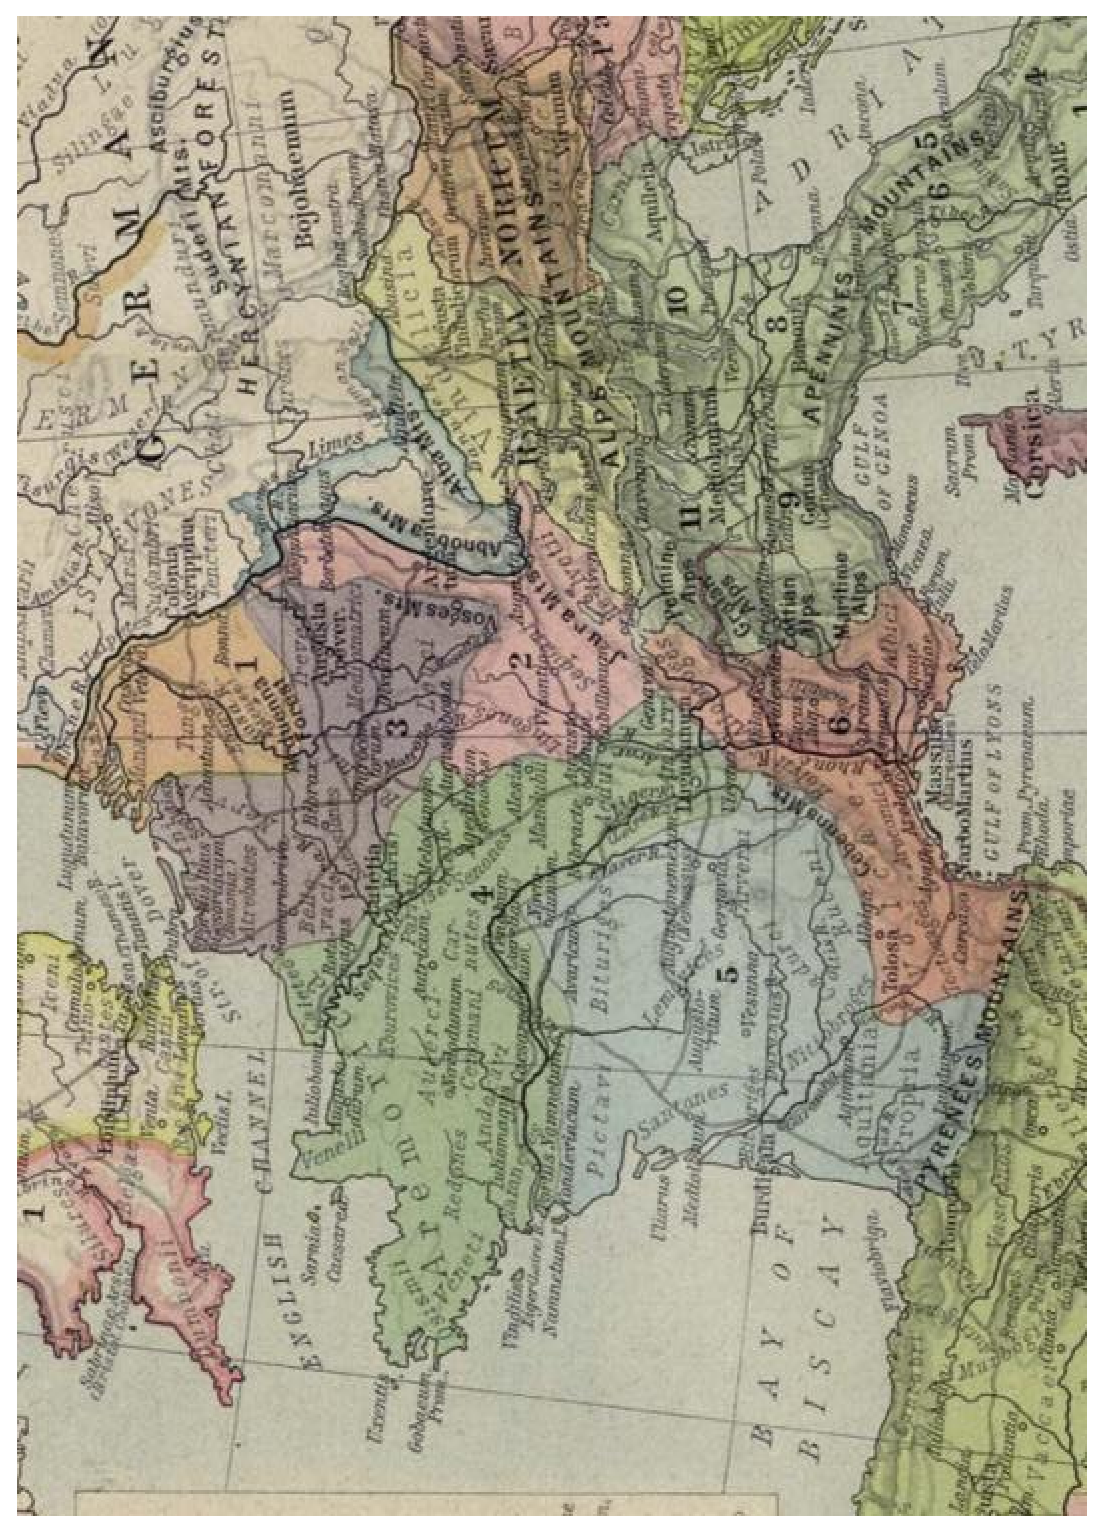
\includegraphics[width=175pt, angle=270]{bilder/Galia}
  \caption{Gallien zur Zeit Caesars}\label{fig_Gallien}
\end{center}
\end{figure}


\begin{table}[htb]
\begin{center}
\begin{tabular}{|l|l|l|}
\hline
Jahr &  Erster Consul & Zweiter Consul\\
\hline \hline
1 & C. Caesar         & L. Aemilius Paullus\\
2 & P. Vinicius       & P. Alfenus Varus\\
3 & L. Aelius Lamia   & M. Servilius\\
4 & Sex. Aelius Catus &  C. Sentius Saturninus\\
5 & L. Valerius Messalla& Cn. Cornelius Cinna \\
suff. & C. Vibius Postumus &  C. Ateius Capito\\
6 & M. Aemilius Lepidus & L. Arruntius\\
\hline
\end{tabular}
 \caption{R�mische Konsulen}\label{tab_Konsulen}
\end{center}
\end{table}


\pagebreak

\section{De Bello Hispaniensi}


%%%%%%%%%%%%%%%%%%%%%%%%%%%%%%%%%%%%%%%%%%%%%%%%%%%%%%%%%%%%%%%%%%%%%%%%%%
%%%%%%%%%%%%%%%%%%%%%%%%%%%%%%% ENDE TEXTTEIL %%%%%%%%%%%%%%%%%%%%%%%%%%%%
%%%%%%%%%%%%%%%%%%%%%%%%%%%%%%%%%%%%%%%%%%%%%%%%%%%%%%%%%%%%%%%%%%%%%%%%%%

\clearpage
\bibliography{references}
\bibliographystyle{alphadin}
%\vspace*{\fill}

\clearpage

\listoffigures

\listoftables

%\pagebreak

%\printindex
\end{document}
